\documentclass[hidelinks,11pt,dvipsnames]{article}
% xcolor commonly causes option clashes, this fixes that
\PassOptionsToPackage{dvipsnames,table}{xcolor}
\usepackage[tmargin=1in, bmargin=1in, lmargin=0.8in, rmargin=1in]{geometry}

%%%%%%%%%%%%%%%%%%%%%%%%%%%%%%%%%%%%%%%%%%%%%%%%%%%%%%%%%%%%%%%%%%%%
%%% For inkscape-figures
%%% Assumes the following directory structure:
%%% master.tex
%%% figures/
%%%     figure1.pdf_tex
%%%     figure1.svg
%%%     figure1.pdf
%%%%%%%%%%%%%%%%%%%%%%%%%%%%%%%%%%%%%%%%%%%%%%%%%%%%%%%%%%%%%%%%%%%%
%\usepackage{import}
\usepackage{pdfpages}
\usepackage{transparent}

\newcommand{\incfig}[2][1]{%
    \def\svgwidth{#1\columnwidth}
    \import{./figures/}{#2.pdf_tex}
}

\pdfsuppresswarningpagegroup=1

% enable synctex for inverse search, whatever synctex is
\synctex=1
\usepackage{float,macrosabound,homework,theorem-env}
\usepackage{microtype}


% font stuff
\usepackage{sectsty}
\allsectionsfont{\sffamily}
\linespread{1.1}

% bibtex stuff
\usepackage[backend=biber,style=alphabetic,sorting=anyt]{biblatex}
\addbibresource{main.bib}

% colored text shortcuts
\newcommand{\blue}[1]{\color{MidnightBlue}{#1}}
\newcommand{\red}[1]{\textcolor{Mahogany}{#1}}
\newcommand{\green}[1]{\textcolor{ForestGreen}{#1}}


% use mathptmx pkg while using default mathcal font
\DeclareMathAlphabet{\mathcal}{OMS}{cmsy}{m}{n}

% fixes the positioning of subscripts in $$ $$
\renewcommand{\det}{\operatorname{det}}

\usetikzlibrary{positioning, arrows.meta}
\newcommand{\here}[2]{\tikz[remember picture]{\node[inner sep=0](#2){#1}}}

%%%%%%%%%%%%%%%%%%%%%%%%%%%%%%%%%%%%%%%%%%%%%%%%%%%%%%%%%%%%%%%%%%%%%
%%% Entry Counter
%%%%%%%%%%%%%%%%%%%%%%%%%%%%%%%%%%%%%%%%%%%%%%%%%%%%%%%%%%%%%%%%%%%%%
\newcounter{entry-counter}
\newcommand{\entry}[1]
{
	\addtocounter{entry-counter}{1}
    \tchap{Entry \arabic{entry-counter}}
	%\addcontentsline{toc}{section}{Entry \arabic{entry-counter}: #1}
	\vspace{-1.5em}
    \begin{center}
		\small \emph{Written: #1}
    \end{center}
}

\usepackage{titling}
\renewcommand\maketitlehooka{\null\mbox{}\vfill}
\renewcommand\maketitlehookd{\vfill\null}


\usepackage{caption}
\usepackage{tikz}
\usetikzlibrary{positioning,calc,intersections,through,backgrounds, shapes.geometric, decorations.markings,arrows}

\def\sset{\subseteq}
\def\iso{\cong}
\def\gend#1{\langle #1\rangle}

\newcommand{\rightoverleftarrow}{%
  \mathrel{\vcenter{\mathsurround0pt
    \ialign{##\crcr
      \noalign{\nointerlineskip}$\longrightarrow$\crcr
      \noalign{\nointerlineskip}$\longleftarrow$\crcr
    }%
  }}%
}

\newcommand\makesphere{} % just for safety
\def\makesphere(#1)(#2)[#3][#4]{%
  % Synopsis
  % \makesphere[draw options](center)(initial angle:final angle:radius)
  \shade[ball color = #3, opacity = #4] #1 circle (#2);
  \draw #1 circle (#2);
  \draw ($#1 - (#2, 0)$) arc (180:360:#2 and 3*#2/10);
  \draw[dashed] ($#1 + (#2, 0)$) arc (0:180:#2 and 3*#2/10);
}
% same thing as makesphere but places white background behind
\newcommand\altmakesphere{} % just for safety
\def\altmakesphere(#1)(#2)(#3)[#4][#5]{%
  % Synopsis
  % \makesphere[draw options](center)(initial angle:final angle:radius)
  \draw [fill=white!30] #1 circle (#2);
  \shade[ball color = #4, opacity = #5] #1 circle (#2);
  \draw #1 circle (#2);
  \draw ($#1 - (#2, 0)$) arc (180:360:#2 and 3*#2/10);
  \draw[dashed] ($#1 + (#2, 0)$) arc (0:180:#2 and 3*#2/10);
  \node at #1 {#3};
}

\begin{document}
\pagestyle{empty}
	\LARGE
\begin{center}
	Algebraic Topo logy Homework 2 \\
	\Large
	Isaac Martin \\
    Last compiled \today
\end{center}
\normalsize
\vspace{-4mm}
\hru

\tchap{Problems from 1.2}
\begin{homework}[e]
  \prob[\textsc{Exercise 1.2.1.}] Show that the free product $G \ast H$ of nontrivial groups $G$ and $H$ has trivial center, and that the only elements of $G \ast H$ of finite order are the conjugates of finite-order elements of $G$ and $H$.
  \begin{prf}
    Recall that two elements of $G\ast H$ are equal if and only if their reductions are identical. We use this fact without comment.

    Suppose that $g \in G$ and $h \in H$ are both nontrivial elements. Then both $ghg^{-1}$ and $h$ are reduced in $G\ast H$, and hence are not equal as they are of different lengths. This means $gh \neq hg$ for all nontrivial elements $g\in G$ and $h \in H$.

    Now suppose we have some reduced word $w_1w_2...w_n \in G\ast H$ where $w_i \in G \cup H$ for $1\leq i\leq n$ and $n \geq 2$. Again let $g \in G$ and $h \in H$ be reduced words. We have four cases to consider.
    \begin{enumerate}[(1)]
      \item If $w_1,w_k \in G$, then $hw$ and $wh$ are both reduced and are hence not equal.
      \item If $w_1,w_k \in H$, then $gw$ and $wg$ are both reduced and are hence not equal.
      \item If $w_1 \in G$ and $w_k \in H$, then $w_2 \in H$ by the assumption that $w$ is reduced. Hence both $gw_2...w_k$ and $wg$ are reduced, and since $k\geq 2$, we have that $gw \neq wg$.
      \item If $w_1 \in H$ and $w_k \in G$, then $w_2 \in G$ and we get $hw \neq wh$ by the same argument as above.
    \end{enumerate}
    Thus, every nontrivial element of $G\ast H$ fails to commute with some other element, meaning the center of $G\ast H$ is trivial.

    We now show that the only elements of $G*H$ are the conjugates of finite-order elements of $G$ and $H$. Let $w \in G*H$ be finite order, i.e. assume $w^k = 1$ where $1$ is the empty word for some $k \in \bN$. 
    
    First, notice that $w$ must have an odd number of letters. If $w = w_1...w_{2n}$ is reduced, then $w_1$ and $w_{2n}$ belong to different groups, and therefore $w^2 = w_1...w{2n}w_1...w{2n}$ is also reduced. Successive multiplication of $w$ with itself will only make the word longer. $w$ must therefore have an odd number of elements in order to reduce upon successive multiplication. Thus the reduced form of $w$ is $w_1...w_{2n+1}$. 
    
    As previously noted, we need $w$ to shrink upon successive products. This means that $w_1$ and $w_{2k+1}$ must multiply to $1$ in either $H$ or $G$, i.e. $w_1 = w_{2n+1}^{-1}$. Similarly, $w_2 = w_{2n}^{-1}$, $w_3 = w_{2n-1}^{-1}$, and $w_n = w_{n+2}^{-1}$. This observation means that 
    \begin{equation*}
        (w_1...w_n)^{-1} = w_n^{-1}...w_1{-1} = w_{n+2}...w_{2n+1}.
    \end{equation*}
    Therefore 
    \begin{equation*}
        w = (w_1...w_n)w_{n+1}(w_{n+2}...w_{2n+1})
    \end{equation*}
    and finally,
    \begin{equation*}
        w^k = (w_1...w_n)w_{n+1}^k(w_{n+2}...w_{2n+1}) = 1 
        \implies w_{n+1}^k = 1
    \end{equation*}
    And since $w_{n+1}$ must be an element in either $H$ or $G$, we conclude that $w$ is the conjugate of some finite order element in $G$ or $H$.


  \end{prf}
  \prob[\textsc{Exercise 1.2.2.}] Let $X \subseteq \bR^m$ be the union of convex open sets $X_1,...,X_n$ such that $X_i \cap X_j \cap X_k \neq \emptyset$ for all $i,j,k.$ Show that $X$ is simply connected. 
  \begin{prf}
    We proceed by induction on $n$. If $n = 1$, then $X$ itself is a convex open set and is hence homeomorphic to an open ball in $\bR^m$, so there is nothing to prove. We do the $n = 2$ case too as a warm up, since it features precisely the setup required for Van Kampen's theorem. We can cover $X$ with $X_1$ and $X_2$, each of which is a convex set, such that $X_1 \cap X_2 \neq \emptyset$. The intersection of convex sets is convex (this is a fact I believe I may use) and hence $X_1\cap X_2$ is path-connected. Hence, by Van Kampen, for any $x_0 \in X_1\cap X_2$ we have
    \begin{align*}
      \pi_1(X,x_0) \cong \pi_1(X_1,x_0) \ast \pi_1(X_2,x_0)/N \cong 1 \ast 1/N \cong 1
    \end{align*}
    since both $X_1$ and $X_2$ are simply connected.

    Now suppose the statement of the problem holds for $1,...,n$ and that $X$ is a union of open convex sets $X_1,...,X_{n+1}$ such that $X_i \cap X_j \cap X_k \neq \emptyset$ for distinct $i,j,k$. By the inductive hypothesis the set $Y = X_1 \cup ... \cup X_n \subset X$ is simply connected. To apply Van Kampen we simply need that $Y \cap X_{n+1}$ is path connected. Choose $x,y \in Y \cap X_{n+1}$. First, notice that we may write
    \begin{align*}
      Y \cap X_{n+1} = (X_1 \cap X_{n+1}) \cup ... \cup (X_n \cap X_{n+1}),
    \end{align*}
    so there is some $i$ and $j$ such that $x \in X_i \cap X_{n+1}$ and $y \in X_j \cap X_{n+1}$. By assumption, the intersection
    \begin{align*}
      X_i \cap X_j \cap X_{n+1}
    \end{align*}
    is nonempty, so we may choose some $z \in X_i \cap X_j \cap X_{n+1}$. Because the intersection of convex sets is convex, we may connect $x$ with $z$ in $X_{i}\cap X_{n+1}$ via a line segment $\alpha$ and $z$ with $y$ in $X_j \cap X_{n+1}$ via a line segment $\beta$. The path $\alpha \cdot \beta$ obtained by concatenating these two line segments is then a path from $x$ to $y$, hence $Y \cap X_{n+1}$ is path connected. Applying Van Kampen as before, we get that
    \begin{align*}
      \pi_1(X,x_0) \cong \pi_1(X_1,x_0) \ast \pi_1(X_2,x_0)/N \cong 1 \ast 1/N \cong 1
    \end{align*}
    since both $Y$ and $X_{n+1}$ are simply connected, and we are done.
  \end{prf}
  \prob[\textsc{Exercise 1.2.4}] Let $X \subseteq \bR^3$ be the union of $n$ lines through the origin. Compute $\pi_1(\bR^3 - X)$.
  \begin{prf}
    Set $Y = \bR^3 - X$ and consider the unit sphere $S^2 \subset \bR^3$ and let $\{p_1,...,p_{2n}\}$. Each line through the origin intersects $S^2$ at exactly two points (antipodal points in fact) and hence $X \cap S^2 = \{p_1,...,p_{2n}\}$.

    I first claim that $Y$ deformation retracts onto $S^2 - \{p_1,...,p^2\}$. This is actually not difficult, simply retract each point $y \in Y$ to the surface of $S^2$ along the ray connecting $y$ to the origin in $\bR^3$. This means that
    \begin{align*}
      \pi_1(Y,y_0) \cong \pi_1(S^2 - \{p_1,...,p_{2n}\}).
    \end{align*}
    
    Next, I claim that $S^2 - \{p_1,...,p_{2n}\}$ deformation retracts onto a wedge of $2n - 1$ circles. This again isn't too hard, but does require more description. Without loss of generality, assume that $p_1,...,p_{2n-1}$ all lie on a great circle containing $p_{2n} = N$, the north pole. Around each point $p_i$ with $1\leq i < 2n$ we may place a copy of $S^1$ such that it intersects the loops around its nearest neighbors at exactly one point, giving us a wedge of $2n-1$ copies of $S^1$. The two nearest neighbors to $N$ will intersect only one of these loops each. From the interior of each of these loops in $S^2 - \{p_1,...,p_{2n}\}$ we deformation retract to the outer boundary, and for any point $y \in S^2 - \{p_1,...,p_2n\}$ not contained in one of these loops we deformation retract along the great arc connecting $y$ to $N$ away from $N$. This gives us a deformation retract of $S^2 - \{p_1,...,p_{2n}\}$ to $\bigvee_{i=1}^{2n-1}S^1$, and thus by Proposition 1.17,
    \begin{align*}
      \pi_1(Y,y_0) \cong \pi_1(S^2 - \{p_1,...,p_{2n}\}) \cong \pi_1\left(\bigvee_{i=1}^{2n-1}S^1,y_0\right) \cong \overbrace{\bZ\ast...\ast\bZ}^{\text{$2n-1$ times}} \cong F_{2n-1}.
    \end{align*}
    Hence $\pi_{1}(Y,y_0)$ is isomorphic to the free group in $F_{2n-1}$ generators.
  \end{prf}
  \prob[\textsc{Exercise 1.2.7}] Let $X$ be the quotient space of $S^2$ obtained by identifying the north and south poles to a single point. Put a cell complex structure on $X$ and use this to compute $\pi_1(X)$.
  \begin{prf}
    Take $X^0 = \{\text{pt}\}$, and let the one skeleton $X^1$ consist of a single interval with both endpoints attached to $\text{pt}$. That is, $X^1$ is a circle.

    We obtain $X$ by attaching a single disk to $X^1$ in the following way. Regard $S^1$, the boundary of $D^2$, as a square with sides labeled $a,b,c$ and $d$ starting from the top and moving anticlockwise. Our attaching map $\varphi:S^1 \to X^1$ is defined as follows.
    \begin{enumerate}
      \item Attach $a$ to $X^1$ by wrapping it once clockwise.
        \begin{center}
          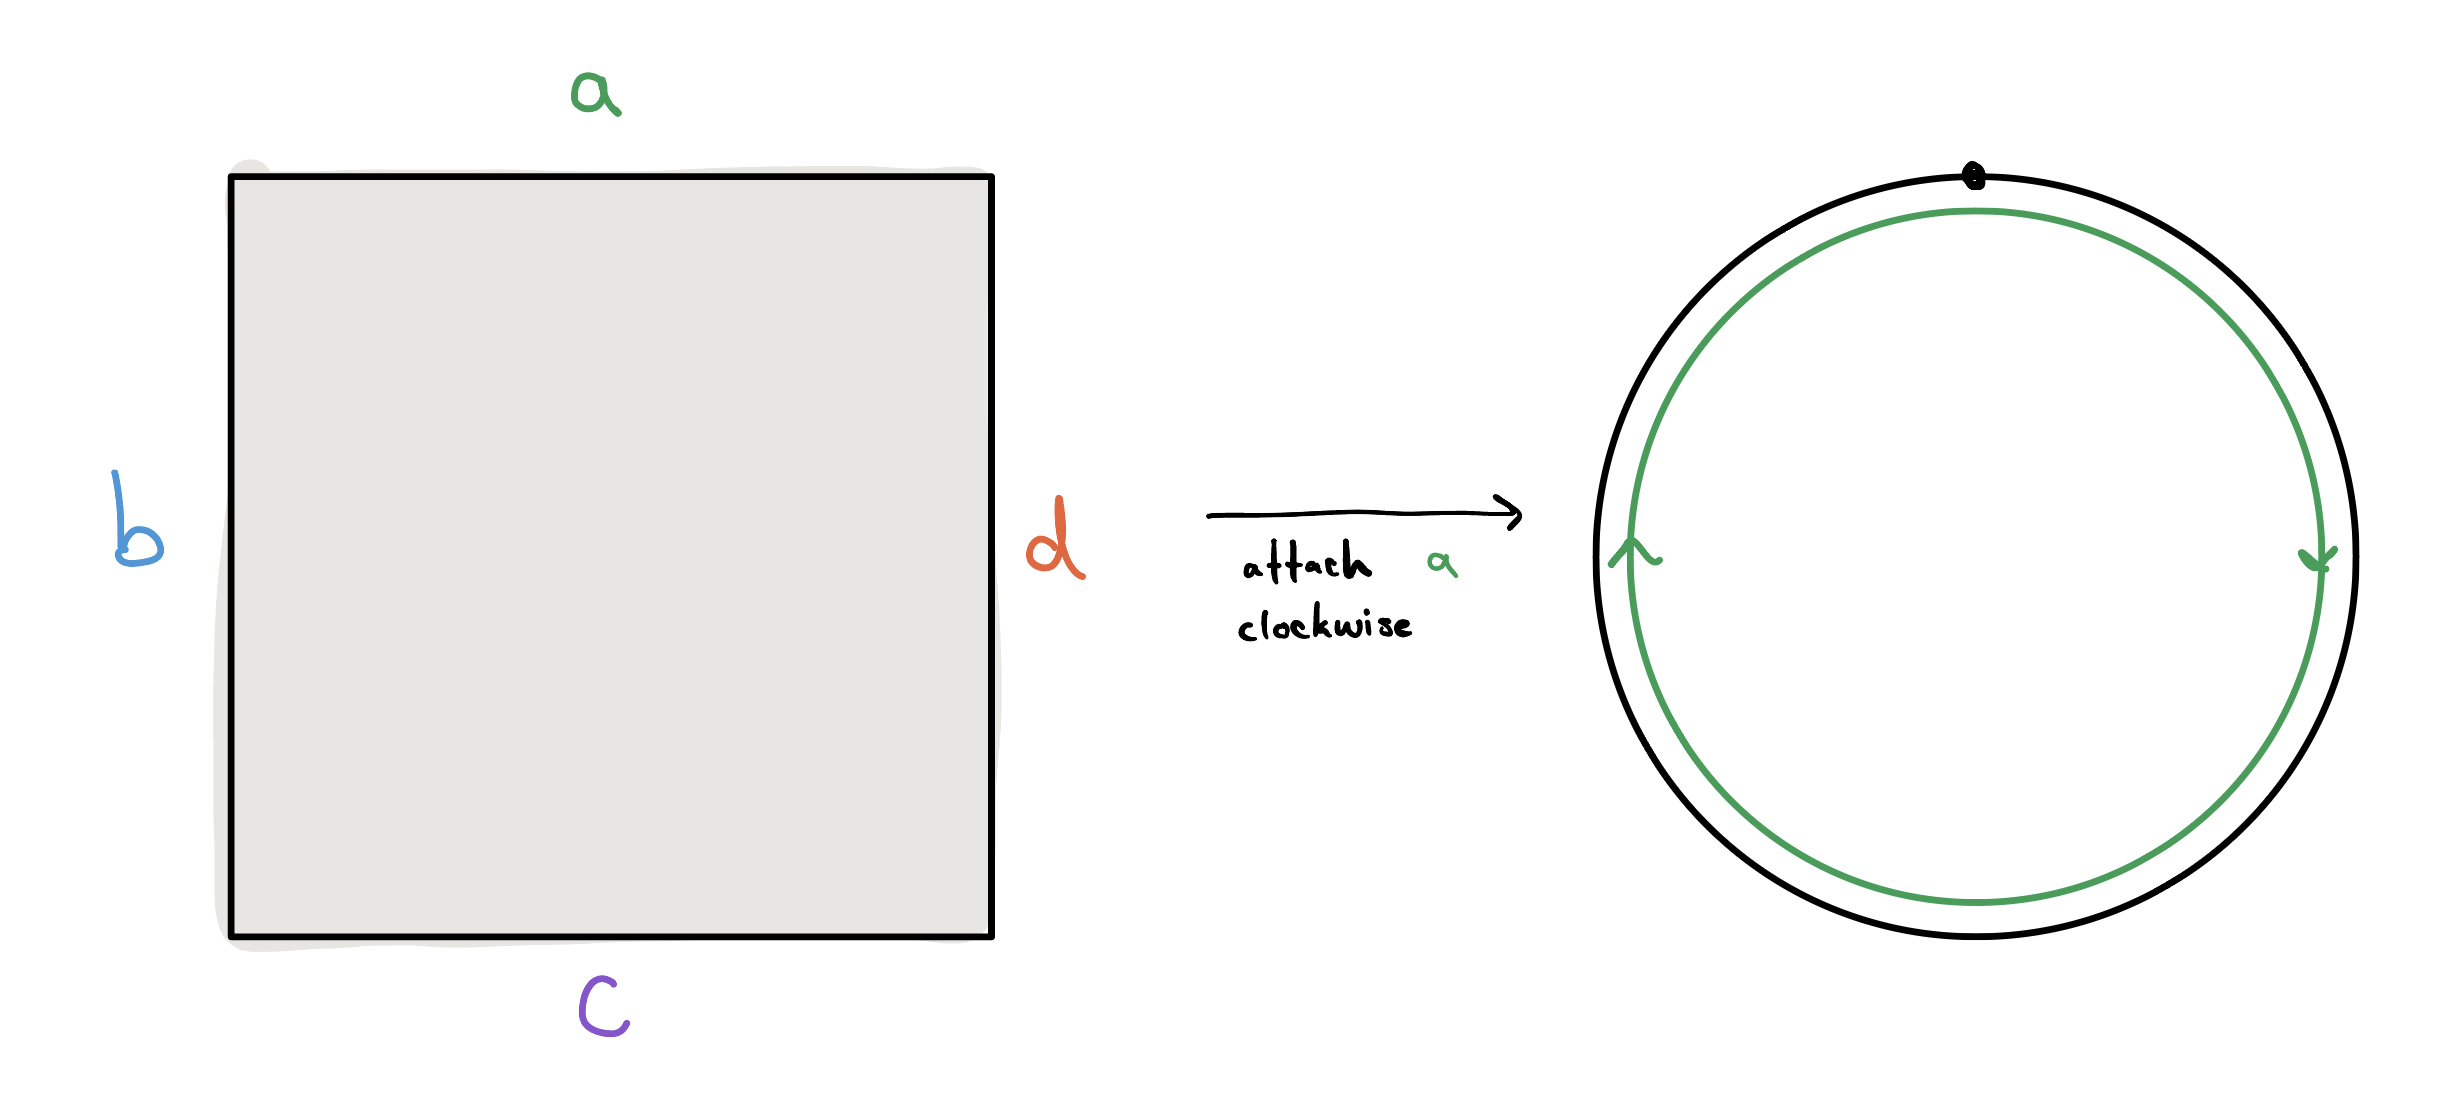
\includegraphics[width=10cm]{figures/hwk3-fig1.jpg}
          \captionof{figure}{Wrap $a$ clockwise around $X^1$}
          \label{fig:prob7.1}
        \end{center}
      \item Collapse $b$ and $d$ to the basepoint $\text{pt}$.
        \begin{center}
          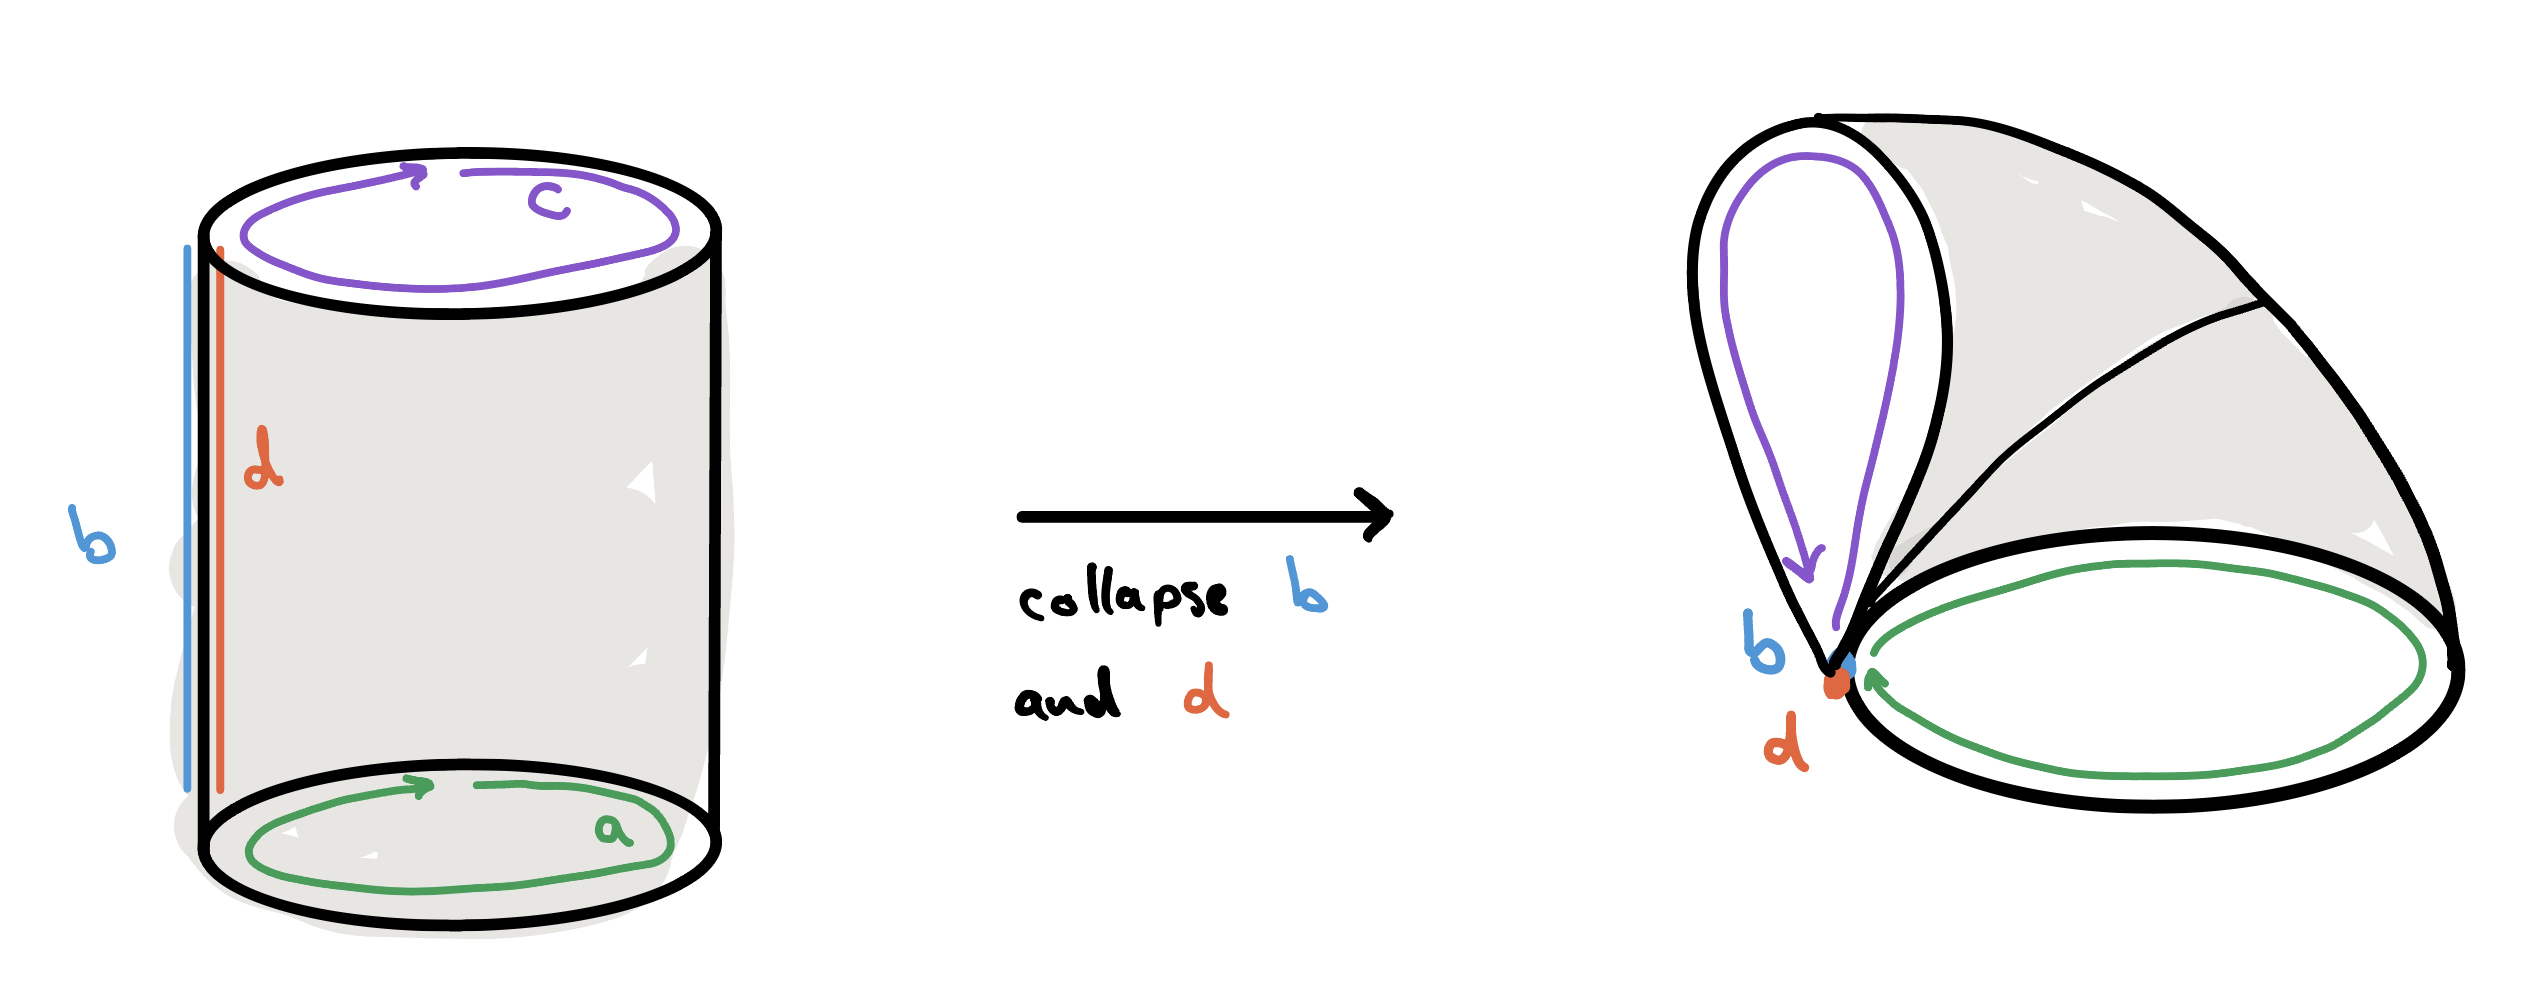
\includegraphics[width=10cm]{figures/hwk3-fig2.jpg}
          \captionof{figure}{Collapse $b$ and $d$ to points}
          \label{fig:prob7.2}
        \end{center}
      \item Attach $c$ by wrapping it once around $X^1$ anticlockwise.
        \begin{center}
          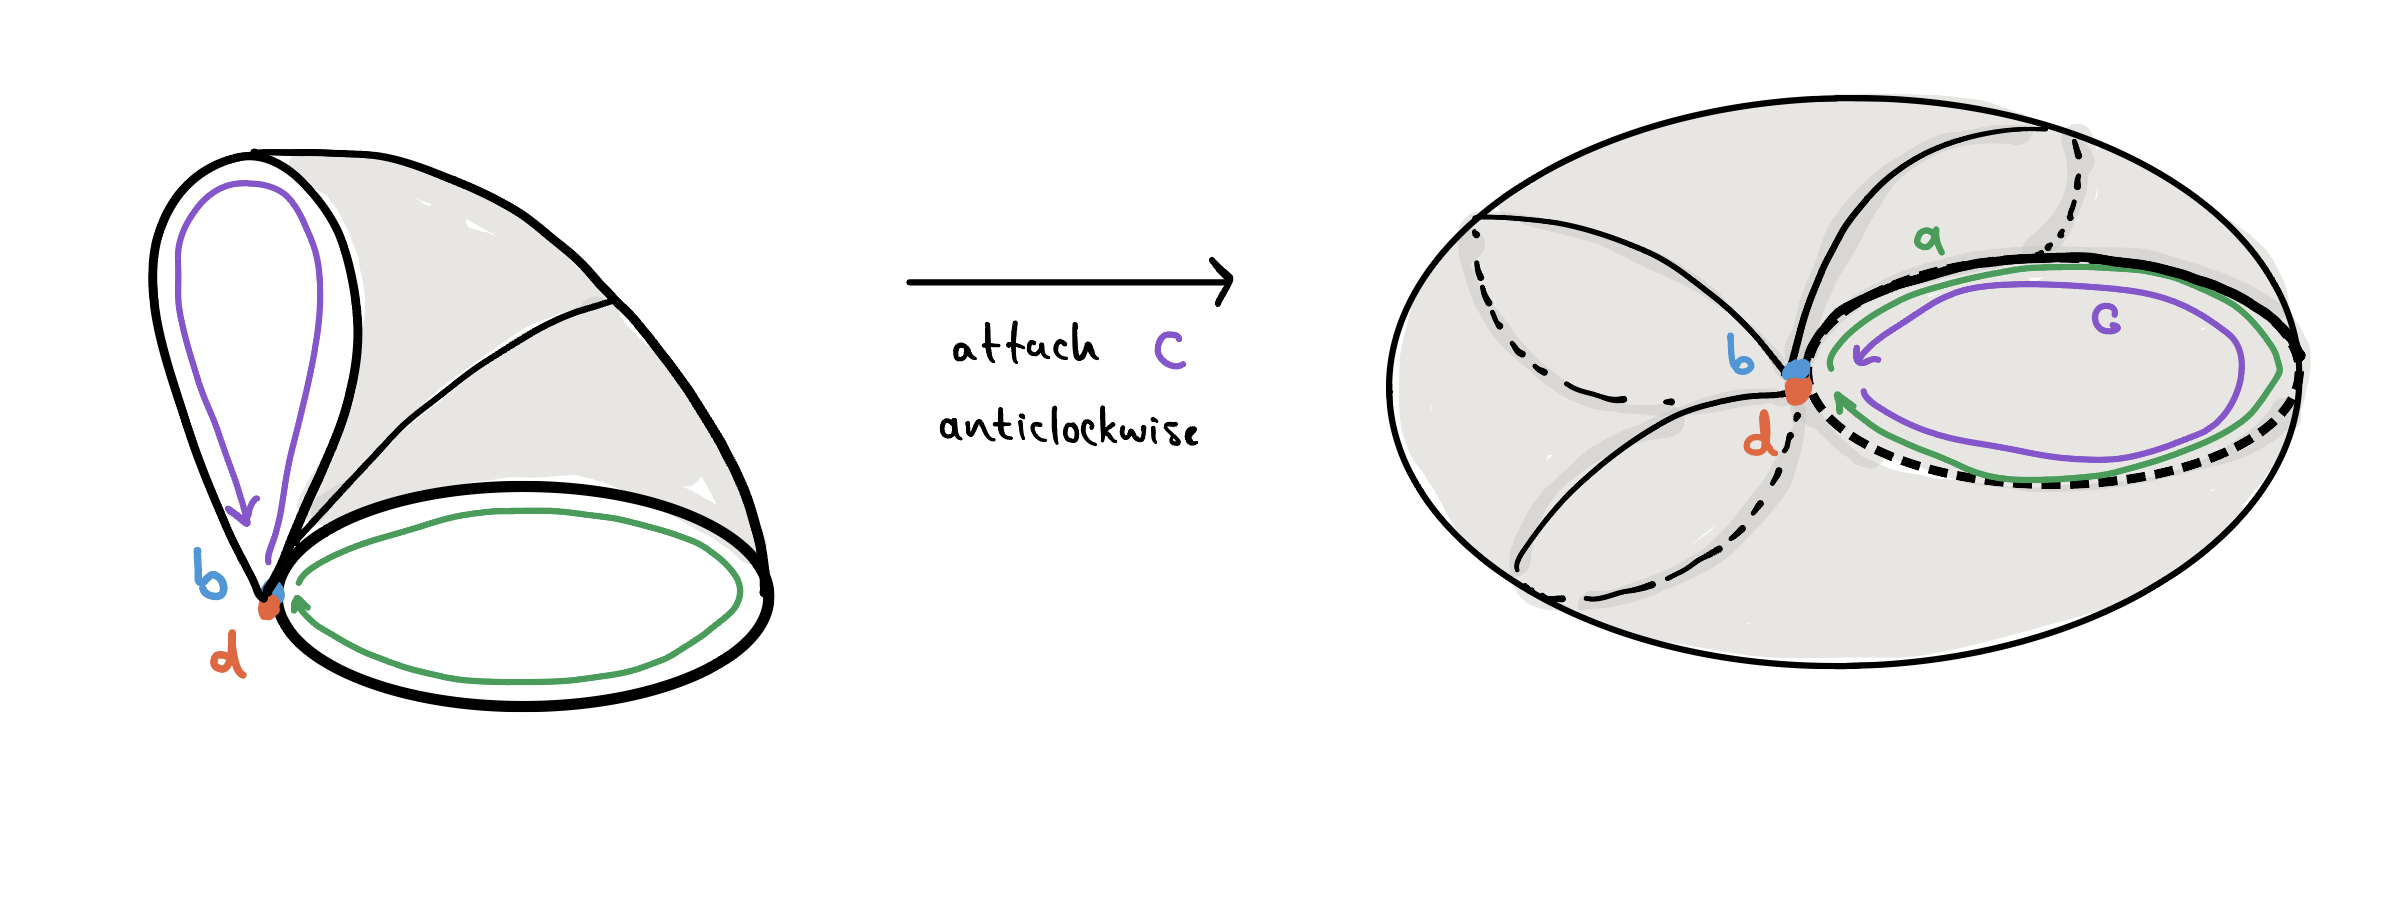
\includegraphics[width=10cm]{figures/hwk3-fig3.jpg}
          \captionof{figure}{Wrap $c$ anticlockwise around $X^1$}
          \label{fig:prob7.3}
        \end{center}
    \end{enumerate}
    Ignore the fact that the inner $X^1$ circle appears to not be filled in Figure \ref{fig:prob7.3}, it is. This process gives a CW-structure on $X$, and we can now compute $\pi_1(X,x_0)$ using Proposition 1.26. The inclusion $X^1 \to X$ induces a surjection $\pi_1(X^1,x_0) \to \pi_1(X,x_0)$ by part (a), whose kernel is generated by conjugations of the attaching map by change of basepoint maps. Choosing $x_0 = \text{pt}$, we then have that the kernel is generated by $[\varphi]$ itself. However, $[\varphi] = 0$ in $\pi_1(X^1,x_0)$ since it is the loop given by rotating once around $X^1$ in both directions. Hence we have an isomorphismk
    \begin{align*}
      \pi_1(X,x_0) \cong \pi_1(X^1,x_0) \cong \bZ.
    \end{align*}
  \end{prf}
  \prob[\textsc{Exercise 1.2.11.}] The \textbf{mapping torus} $T_f$ of a map $f:X \rightarrow X$ is the quotient of $X\times I$ obtained by identifying each point $(x,0)$ with $\left(f(x),1\right)$. In the case $X= S^1 \vee S^1$ with $f$ basepoint preserving, compute a presentation for $\pi_1(T_f)$ in terms of the induced map $f_*:\pi_1(X) \rightarrow \pi_1(X)$. Do the same when $X = S^1 \times S^1$.

\begin{prf}
    We consider first the case where $X = S^1 \vee S^1$. We can express $X$ as a CW-complex with one 0-cell and two 1-cells through the following construction. Let $x_0$ be a 0-cell. Attach the ends of two 1-cells to $x_0$, and we have $X$. 
    
    Now, because $f$ is basepoint preserving, if we take $x_0$ to be our basepoint, $x_0 \mapsto x_0$ which means that under the equivalence relation, $(x_0, 0) \mapsto (x_0, 1)$. As stated in Hatcher, we can regard $T_f$ as the construction of $X \vee S^1$ with appropriate cells attached, i.e. as the space obtained by taking every $k$ cell in $X$ and attaching a $k+1$ cell. This is visualized in the diagram below. By Proposition 1.26, we therefore have that $\pi_1(T_f) \cong \pi_1(X \vee S^1)/N$. However, this is precisely the fundamental group from question (8). Thus,
    \begin{equation*}
        \pi_1(T_f) \approx 
        (\bZ * \bZ * \bZ) / 
        \langle aba^{-1}b^{-1}, cdc^{-1}d^{-1} \rangle
    \end{equation*}
    Where $a = f_*(a)$, etc.
    
    \bigskip
    
    We now consider the case where $X = S^1 \times S^1$. This is a torus. We once again regard $T_f$ as the space obtained by attaching appropriate cells to $X \vee S^1$. This time we attach one 3-cell (for the 2-cell of the torus) and two two-cells (for the two 1-cells of the torus). One again, the wedge with $S^1$ is the result of attaching one 1-cell to the basepoint of $X$.
    
    From part (b) of Proposition 1.26, we know that the 3-cell is simply connected and therefore doesn't affect $\pi_1(T_f)$. We therefore obtain almost exactly the same fundamental group as before, except that we have an extra 1-cell. This extra cell causes $a$ and $b$ to commute. Therefore, 
    \begin{equation*}
        \pi_1(T_f) \approx 
        (\bZ * \bZ * \bZ) / 
        \langle aba^{-1}b^{-1}, cdc^{-1}d^{-1} \mid ab = ba \rangle
    \end{equation*}
\end{prf}
\newpage
\begin{figure}[h]
    \centering
    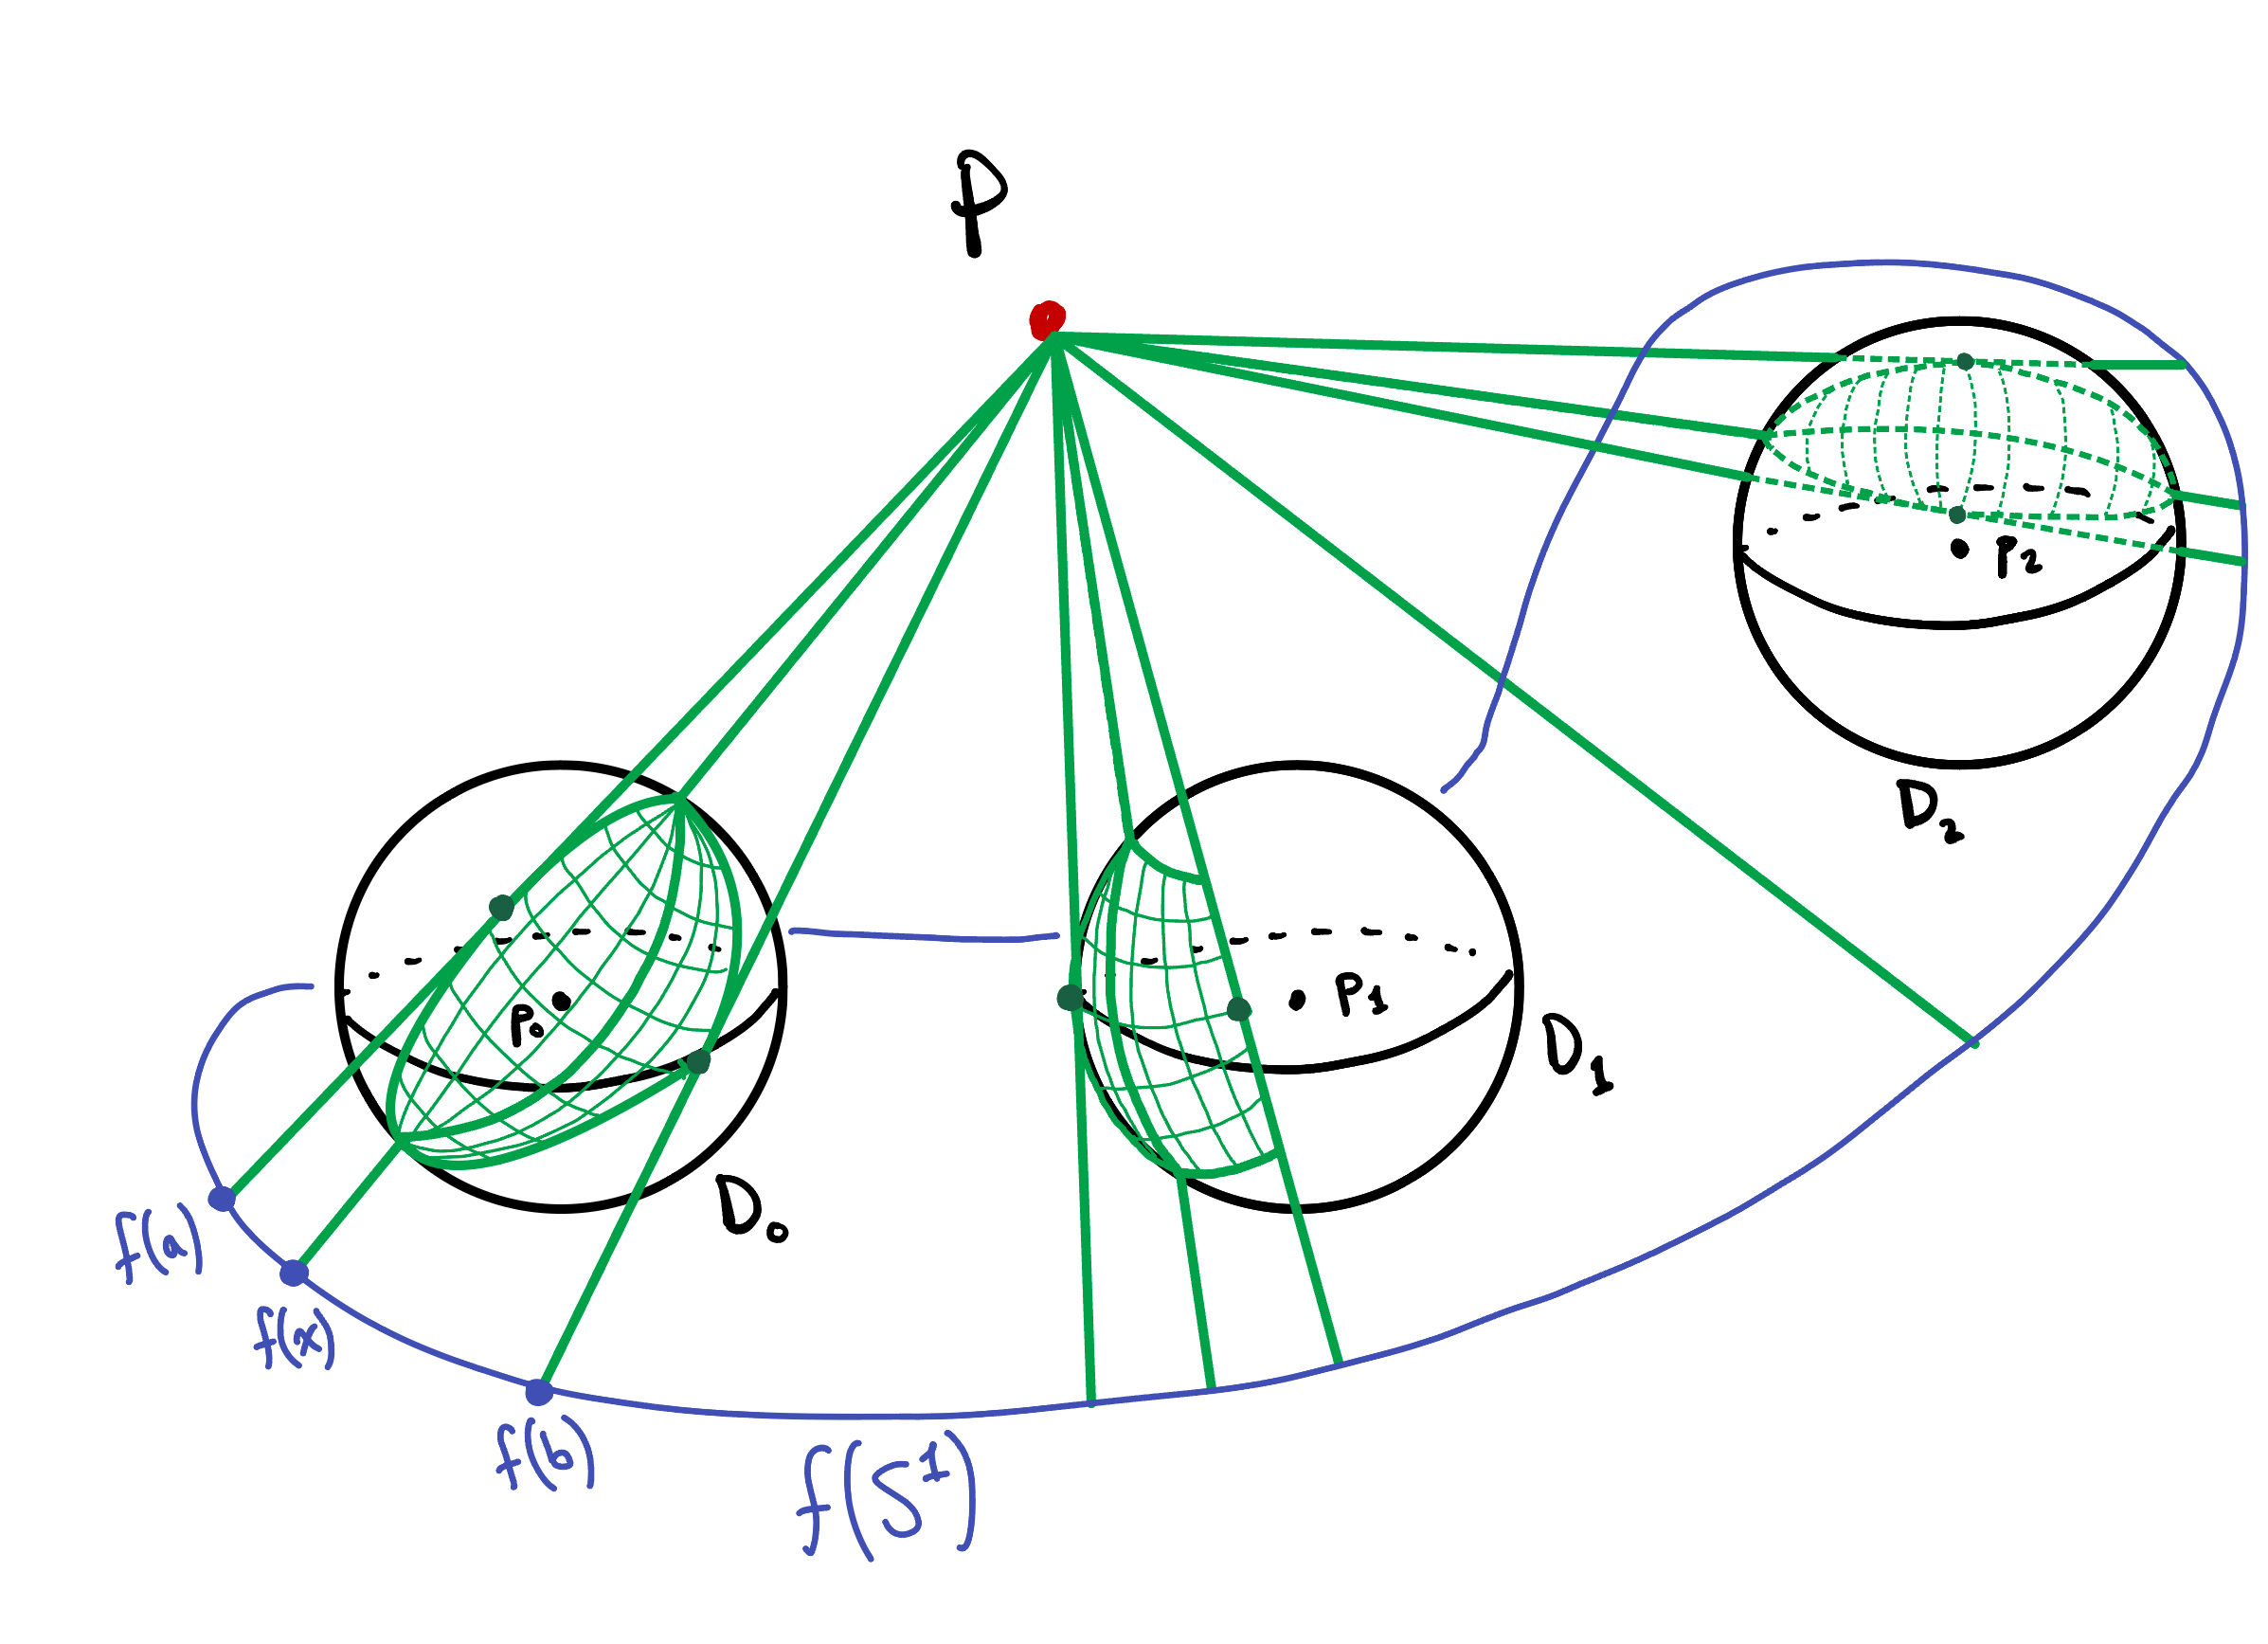
\includegraphics[width=10cm]{./figures/hwk2-fig1.jpg}
    \caption{The homotopy in Case 1}
    \label{fig:case1}
\end{figure}

\end{homework}
\end{document}
